%Copyright 2014 Jean-Philippe Eisenbarth
%This program is free software: you can 
%redistribute it and/or modify it under the terms of the GNU General Public 
%License as published by the Free Software Foundation, either version 3 of the 
%License, or (at your option) any later version.
%This program is distributed in the hope that it will be useful,but WITHOUT ANY 
%WARRANTY; without even the implied warranty of MERCHANTABILITY or FITNESS FOR A 
%PARTICULAR PURPOSE. See the GNU General Public License for more details.
%You should have received a copy of the GNU General Public License along with 
%this program.  If not, see <http://www.gnu.org/licenses/>.

%Based on the code of Yiannis Lazarides
%http://tex.stackexchange.com/questions/42602/software-requirements-specification-with-latex
%http://tex.stackexchange.com/users/963/yiannis-lazarides
%Also based on the template of Karl E. Wiegers
%http://www.se.rit.edu/~emad/teaching/slides/srs_template_sep14.pdf
%http://karlwiegers.com


\documentclass{scrreprt}

\usepackage{pdfpages}
\usepackage{listings}
\usepackage[T1]{fontenc}
\usepackage{placeins}
\usepackage{float}
\usepackage{underscore}
\usepackage[bookmarks=true]{hyperref}
\usepackage[utf8]{inputenc}
\usepackage{graphicx}
\usepackage{subfigure}
\usepackage[english]{babel}
\hypersetup{
	bookmarks=false,    % show bookmarks bar?
	pdftitle={Software Requirement Specification},    % title
	pdfauthor={Adam-Ryan},                     % author
	pdfsubject={TeX and LaTeX},                        % subject of the document
	pdfkeywords={TeX, LaTeX, graphics, images}, % list of keywords
	colorlinks=true,       % false: boxed links; true: colored links
	linkcolor=blue,       % color of internal links
	citecolor=black,       % color of links to bibliography
	filecolor=black,        % color of file links
	urlcolor=blue,        % color of external links
	linktoc=page            % only page is linked
}%
\def\myversion{1 }
\date{}
%\title
\usepackage{hyperref}
\begin{document}
	
	\begin{flushright}
		\rule{16cm}{5pt}\vskip1cm
		\begin{bfseries}
			\Huge{Tutorial 7\\}
			\vspace{1.9cm}
			for\\
			\vspace{1.9cm}
			Data Mining - Tutorial 7
			\vspace{1.9cm}
			\LARGE{Version \myversion}\\
			\vspace{1.9cm}
			Adam Ryan (14395076)\\
			\vspace{1.9cm}
			COMP40370\\
			\vspace{1.9cm}
			\today\\
		\end{bfseries}
	\end{flushright}
	
	\tableofcontents

	
\chapter{Question 1}

\section{Part 1}\label{E1Q1}
I visualise the dataframe using matplotlib. The result is below. We see three clusters present broadly in the top left, bottom left, and top right of the plot.

\begin{figure}[h!]
	\centering
	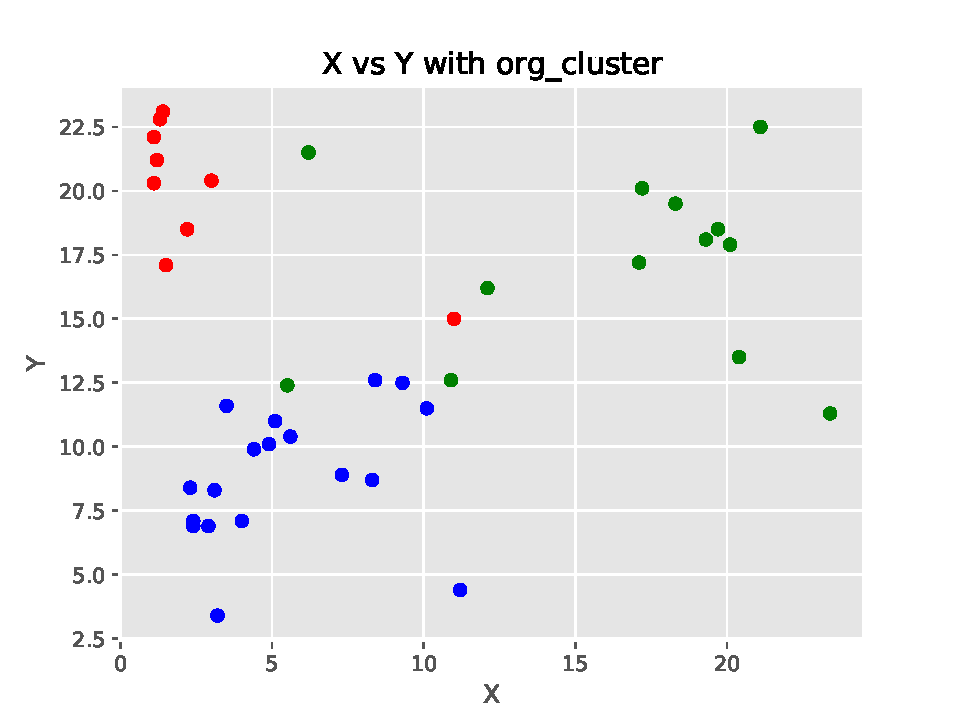
\includegraphics[width=0.5\linewidth]{question_1_1.pdf}
\end{figure}

\section{Part 2}\label{E1Q2}
I write a clustering and scoring function, and plot the intertia using the resulting dictionary. We see the elbow point is at three clusters from the graph, as the resultant gains slow considerably after this point. This suggests that we should choose three clusters for the dataset.
\begin{figure}[h!]
	\centering
	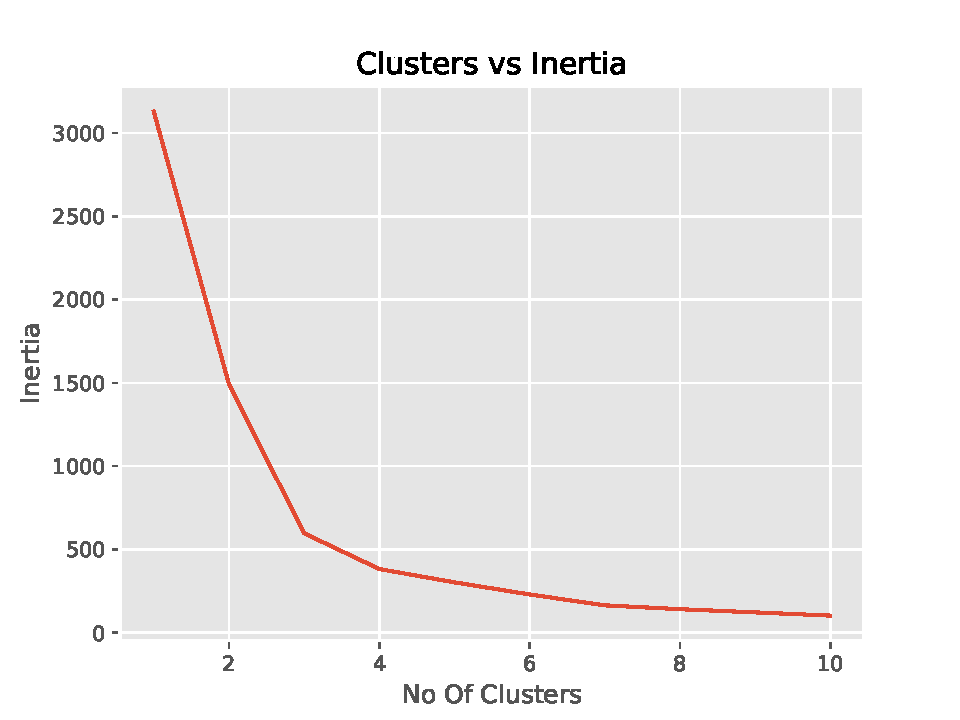
\includegraphics[width=0.5\linewidth]{question_1_2.pdf}
\end{figure}

\section{Part 3}\label{E1Q3}
I calculate the rand index and silhouette score using sklearn's metrics. For three clusters, I get the values below:
\begin{itemize}
	\item[rand] $= 0.8666...$
	\item[silhouette] $= 0.6093075207861811$
\end{itemize}

\section{Part 4}\label{E1Q4}
I add on this column by taking the result from my clustering dictionary.

\section{Part 5}\label{E1Q5}
I plot the centroids and new clusters using matplotlib and force the label colourings to match the original clusters for plotting purposes (I do not relabel these in the dataframe however the mapping is present in the colouring function if required). The centers are the markers in the graph with the '+' symbol in the same colour as the rest of that cluster.
\begin{figure}[h!]
	\centering
	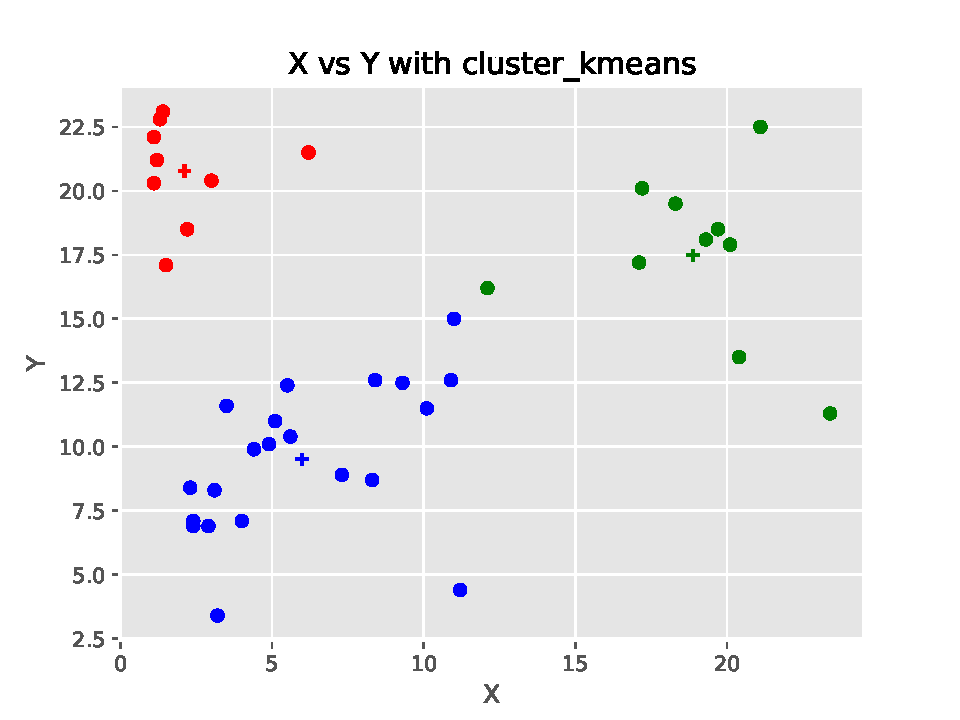
\includegraphics[width=0.5\linewidth]{question_1_5.pdf}
\end{figure}

\newpage
\chapter{Question 2}

\section{Part 1}\label{E2Q1}
I discard the columns by taking the set difference of the original columns and columns to discard, and taking the dataframe with the remaining columns.

\section{Part 2}\label{E2Q2}
I modify the clustering dictionary created for question 1 and modify it for the new parameters and dataset in question 2. This part corresponds  the first set of parameters in run\_config of '[5,5,100]'. I label the column appropriately in the dataframe.

\section{Part 3}\label{E2Q3}
I modify the clustering dictionary created for question 1 and modify it for the new parameters and dataset in question 2. This part corresponds with the second set of parameters in run\_config of '[5,100,100]'. I label the column appropriately in the dataframe.

\section{Part 4}\label{E2Q4}
We see that only nine labels match exactly if we compare the assigned labels between config1 and config2. Changing n\_init alters how many different initial centroid starting positions are used by the kmeans++ algorithm, and the best run by inertia is then returned.

\section{Part 5}\label{E2Q5}
I modify the clustering dictionary created for question 1 and modify it for the new parameters and dataset in question 2. This part corresponds with the third set of parameters in run\_config of '[3,10,100]'. I label the column appropriately in the dataframe. One point of note is it doesn't say what to use for the second parameter in the question, so I've chosen the sklearn default value of 10.

\section{Part 6}\label{E2Q6}
With the following configuration values, the highest silhouette score is obtained with three clusters, while the lowest inertia is obtained in the second configuration. The precise scores identified are described below. 
\begin{itemize}
	\item config1: 5\_5\_100    : Silhouette: 0.33509164287562027
	\item config2: 5\_100\_100  : Silhouette: 0.3601346535452705
	\item config3: 3\_10\_100   : Silhouette: 0.46430924739274937
\end{itemize}
\begin{itemize}
	\item config1: 5\_5\_100    : Inertia: 221721.30216033317
	\item config2: 5\_100\_100  : Inertia: 221177.56684887334
	\item config3: 3\_10\_100   : Inertia: 349679.2299669071
\end{itemize}
Based on these results, my recommendation would be that config2 appears to produce the most accurate clusters as the inertia is the lowest indicating the points are most tightly clustered, however the improvement is only minor compared to config1.

\newpage
\chapter{Question 3}

\section{Part 1}\label{E3Q1}
I discard ID, create clusters using SKLearn, and generate the plot below. We can clearly see there are five (or six depending on your view of the middle left shape) shapes in the dataset with some random points outside of these shapes falling into a final additional cluster. KMeans fails to appropriately capture this behaviour in the classification as it instead broadly creates clusters depending where in the plot the point falls, missing the graphical shape behaviour of the data.
\begin{figure}[h!]
	\centering
	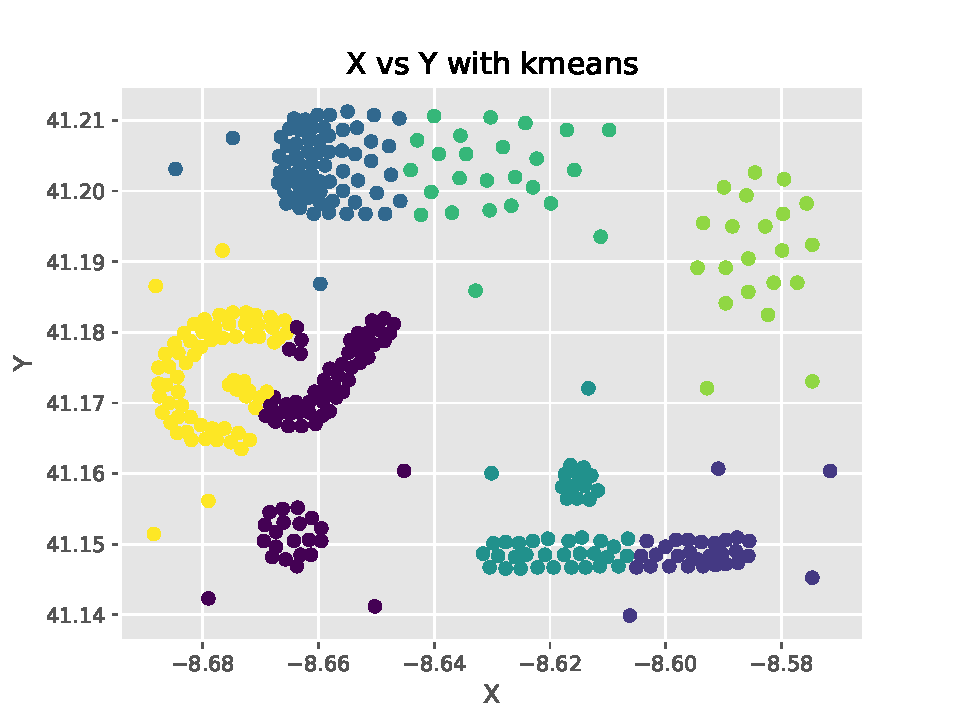
\includegraphics[width=0.5\linewidth]{question_3_1.pdf}
\end{figure}


\section{Part 2}\label{E3Q2}
Plot as above in \ref{E3Q1}

\section{Part 3}\label{E3Q3}
I do this using epsilon=0.04 instead of 0.4 Using 0.4 produced only a single label, while the test case seems to require a value of 0.04 to match the assertion in the test script. I use the minmax scaler to scale things in a range of 0 to 1 as part of my clustering function, and add the dbscan1 results to my dataframe. The following plot is generated:
\begin{figure}[h!]
	\centering
	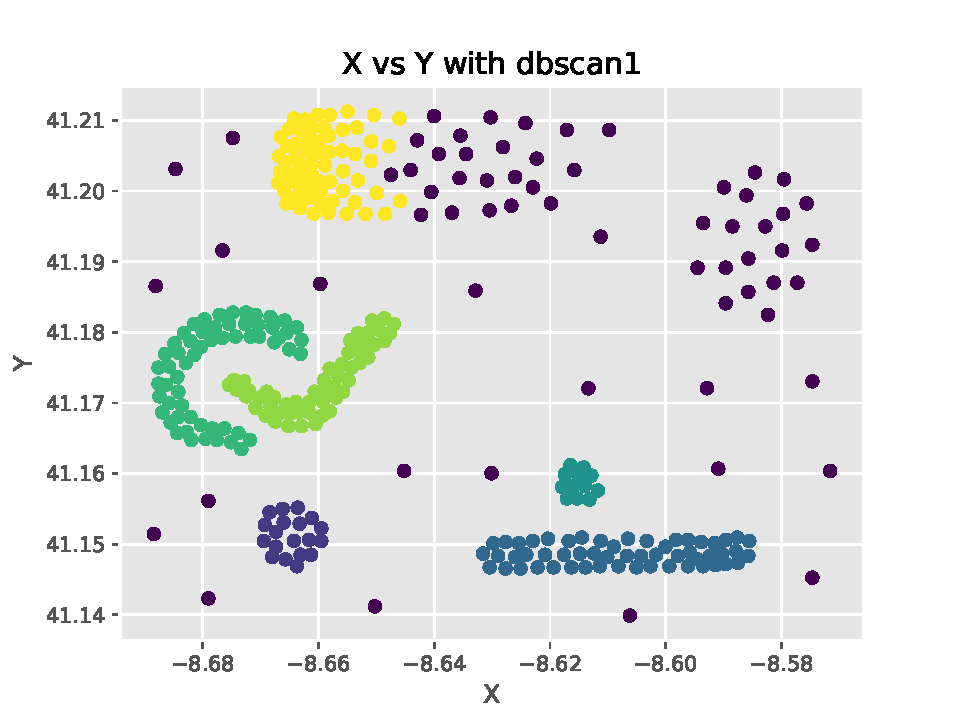
\includegraphics[width=0.5\linewidth]{question_3_2.pdf}
\end{figure}


\section{Part 4}\label{E3Q4}
I do this using epsilon=0.08. I use the minmax scaler to scale things in a range of 0 to 1 as part of my clustering function, and add the dbscan2 results to my dataframe. The following plot is generated:
\begin{figure}[h!]
	\centering
	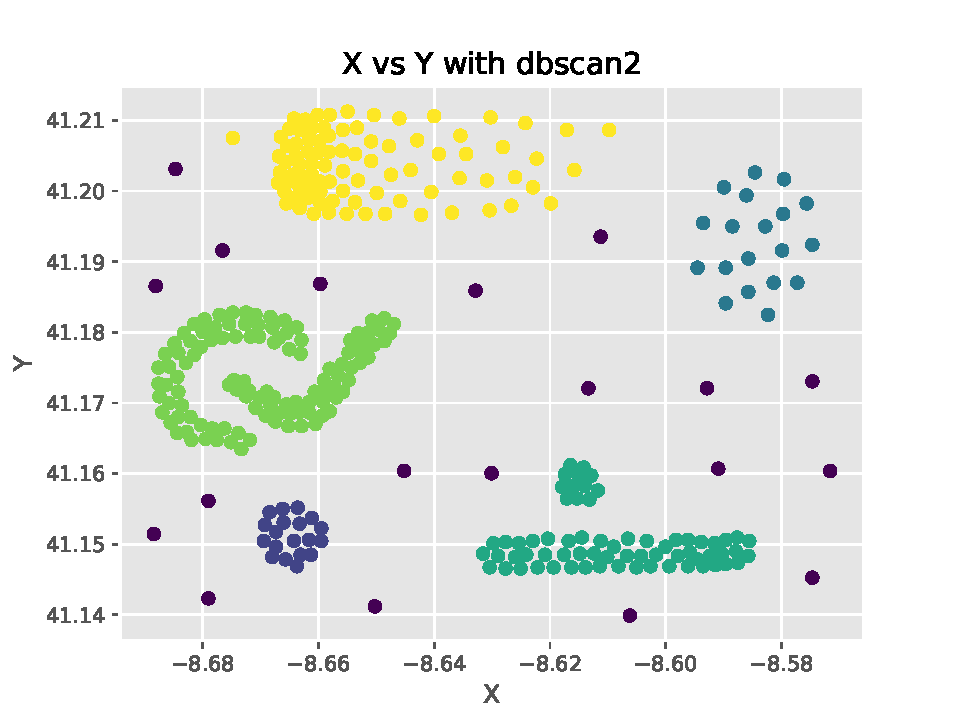
\includegraphics[width=0.5\linewidth]{question_3_3.pdf}
\end{figure}

\section{Part 5}\label{E3Q5}
I save the file using pandas.

\pagebreak
\section{Part 6}\label{E3Q6}
Comparing the three graphs obtained in the preceeding question, we see that dbscan2 produces the most accurate clustering result. kmeans fails to account for the 'shape' of the clusters and instead clusters based on their position in the graph (which makes sense given how kmeans is based on the generation of balls with a given metric). DBScan1 is an improvement however it fails to appropriately identify that the 'circle tick' shape on the mid-left of the plot is part of the same cluster, and has difficulties with the shape on the top and the random points. dbscan2 is clearly the best result as it captures the different shapes present in the data and appropriately groups the 'random' data together. This is sensible as dbscan is specifically designed to identify clusters with a distinctive shape and noise present. The difference between kmeans and dbscan is that while kmeans produces convex balls of a given metric around a centroid, dbscan works by assigning points as core points, (which contain at least as many points as the minimum number of points in a ball of a given metric of radius epsilon centered on a given core point), border points (which are themselves contained in a ball surrounding a core point but are not themselves a core point), and outliers which don't fall into the above. The process of creating neighbourhoods around each point works to identify areas of high and low density and cluster them together. By expanding the epsilon in dbscan2, the trailing points in the top shape fall within core and border points clustering them together (whereas epsilon is too tight in dbscan1 to capture them together) and likewise for the shape on the mid-left. This the key reason why increasing epsilon results in better behaviour between dbscan1 and dbscan2.
\begin{figure}[h!]
	\centering
	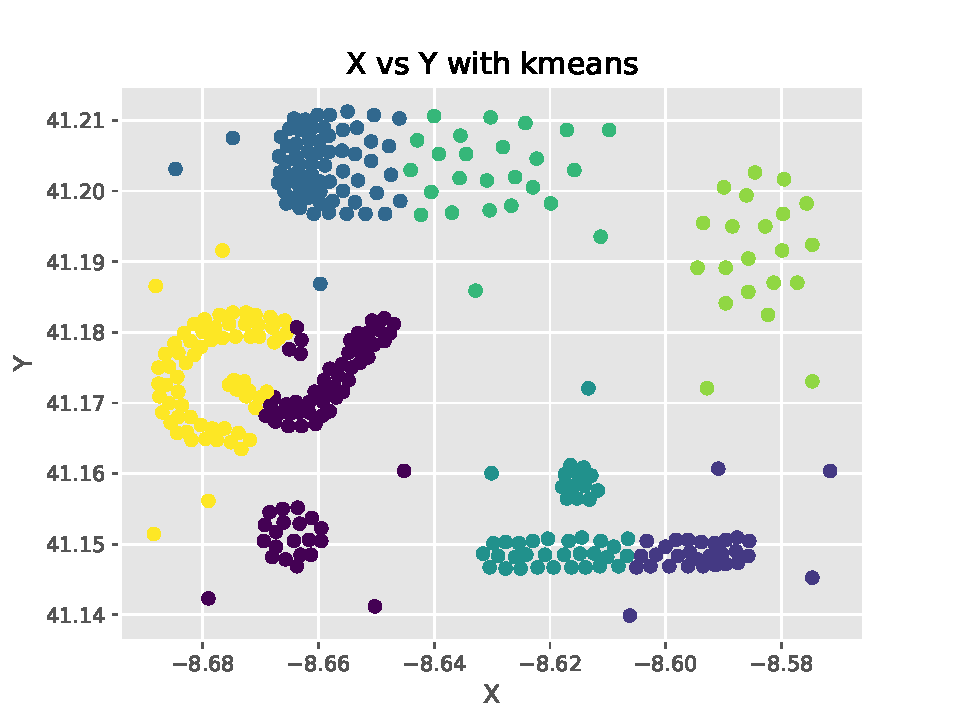
\includegraphics[width=0.3\linewidth]{question_3_1.pdf}
	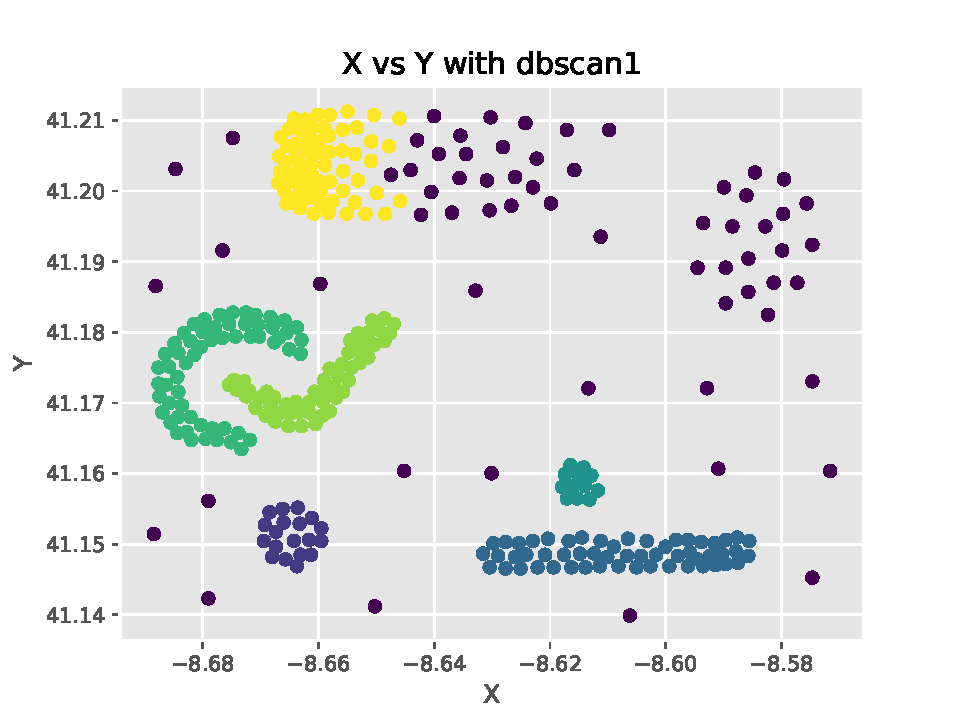
\includegraphics[width=0.3\linewidth]{question_3_2.pdf}
	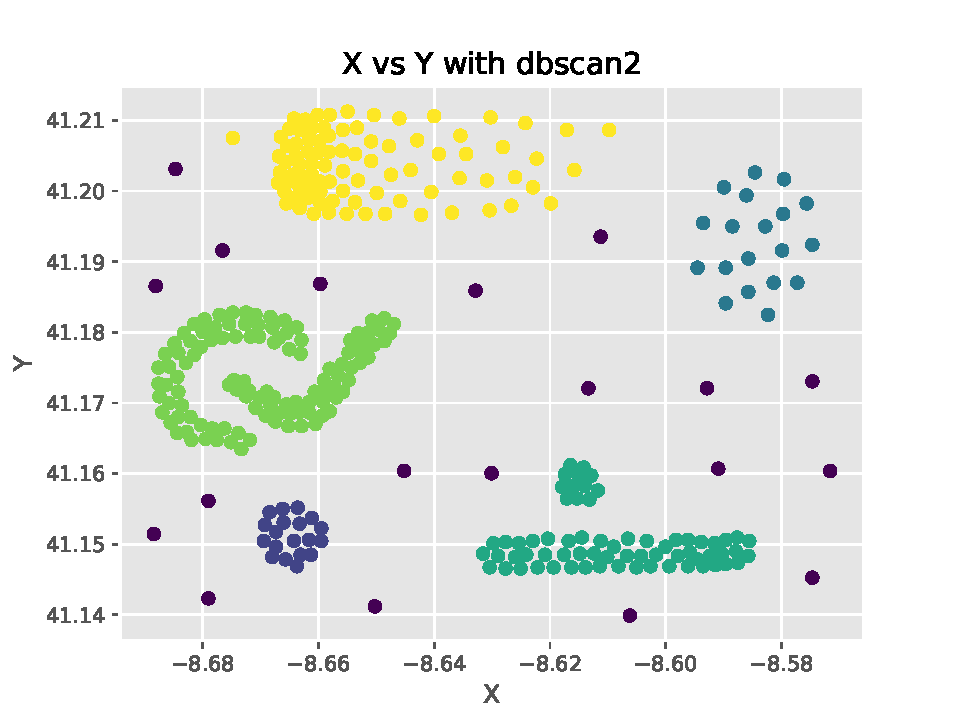
\includegraphics[width=0.3\linewidth]{question_3_3.pdf}
\end{figure}

\end{document}
